
\section*{Problema 02}

\textbf{Ordena las siguientes distribuciones en base de su entropía de Shannon (de menor a mayor). Motiva tu respuesta.}

\begin{figure}[H]
    \centering
    \begin{subfigure}{4cm}
        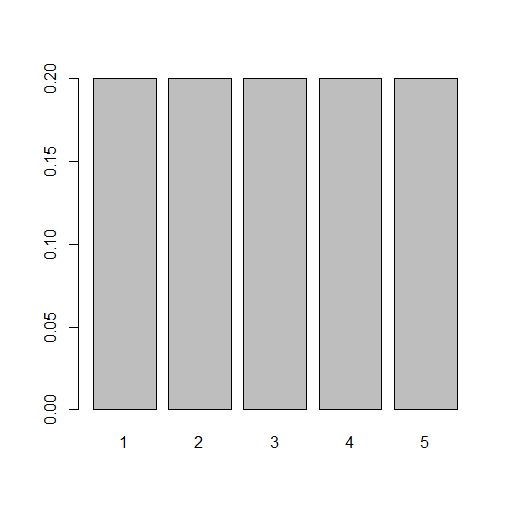
\includegraphics[width=4cm]{Graphics/Problema_02_1.png}
        \caption{Distribución 1}
    \end{subfigure}
    \begin{subfigure}{4cm}
        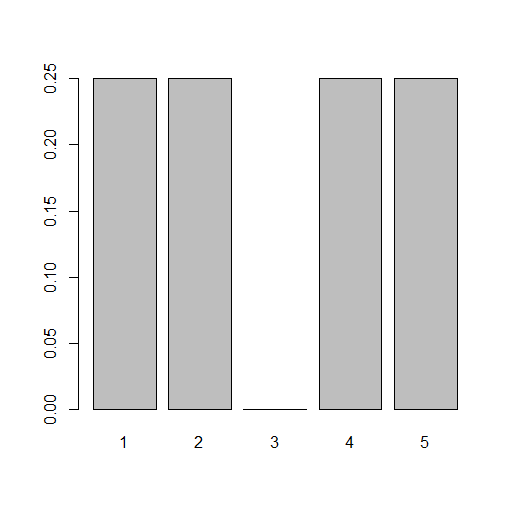
\includegraphics[width=4cm]{Graphics/Problema_02_2.png}
        \caption{Distribución 2}
    \end{subfigure}
    \begin{subfigure}{4cm}
        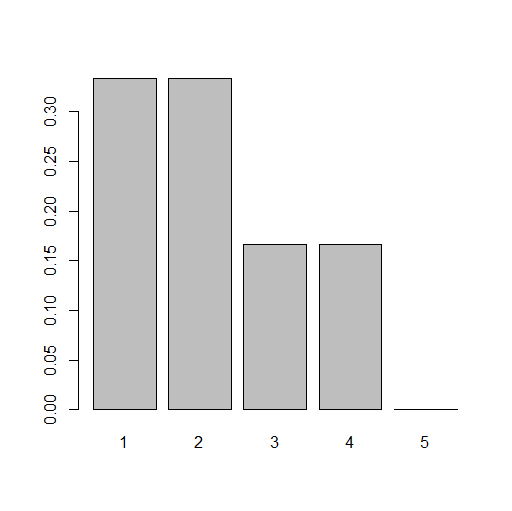
\includegraphics[width=4cm]{Graphics/Problema_02_3.png}
        \caption{Distribución 3}
    \end{subfigure}
    \begin{subfigure}{4cm}
        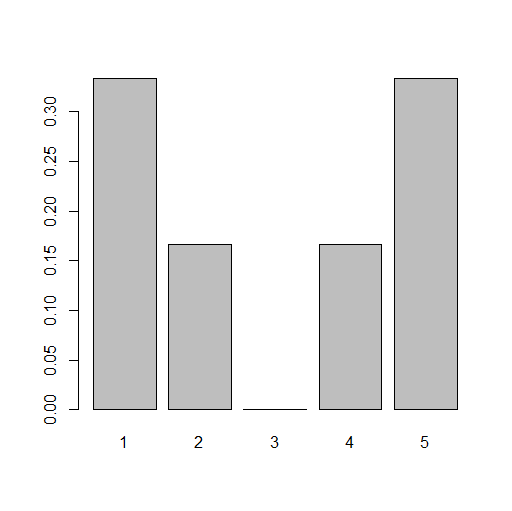
\includegraphics[width=4cm]{Graphics/Problema_02_4.png}
        \caption{Distribución 4}
    \end{subfigure}
    \caption{Diferentes distribuciones.}
    \label{fig:problema_02}
\end{figure}

En la tabla \ref{table:distributions} se encuentran los alores de las distribuciones de la figura \ref{fig:problema_02}.

\begin{table}[H]
    \centering
    \begin{tabular}{cccccc} \hline
        Distribución & 1    & 2    & 3    & 4    & 5    \\ \hline
        1            & 0.20 & 0.20 & 0.20 & 0.20 & 0.20 \\
        2            & 0.25 & 0.25 & 0    & 0.25 & 0.25 \\
        3            & 0.34 & 0.34 & 0.16 & 0.16 & 0    \\
        4            & 0.34 & 0.16 & 0    & 0.16 & 0.34 \\ \hline
    \end{tabular}
    \caption{Valores de las distribuciones mostradas en la figura \ref{fig:problema_02}}
    \label{table:distributions}
\end{table}

Basandonos en los datos, se puede decir que la distribución con mayor entropía es la distribución 1. Esto debido a que todos sus valores contiene la misma probabilidad. Otra afirmación que se puede realizar es que las distribuciones 3 y 4 tienen la misma entropía debido a que tienen una semejanza en su distribución de probabilidades. El cambio es que probabilidad esta asociada a cada valor. Con la información de la tabla \ref{table:distributions} se puede calcular la entropía de Shannon para comprobar lo antes dicho. Los resultados se muestran en la tabla \ref{table:distributions_2}.

\begin{table}[H]
    \centering
    \begin{tabular}{ccccccc} \hline
        Distribución & 1    & 2    & 3    & 4    & 5    & Entropía \\ \hline
        1            & 0.20 & 0.20 & 0.20 & 0.20 & 0.20 & 0.6989   \\
        2            & 0.25 & 0.25 & 0    & 0.25 & 0.25 & 0.6026   \\
        3            & 0.34 & 0.34 & 0.16 & 0.16 & 0    & 0.5732   \\
        4            & 0.34 & 0.16 & 0    & 0.16 & 0.34 & 0.5732   \\ \hline
    \end{tabular}
    \caption{Valores de las distribuciones mostradas en la figura \ref{fig:problema_02} con sus respectivos valores de entropía.}
    \label{table:distributions_2}
\end{table}

Con esto podemos afirmar que el orden de menor a mayo entropía es distribución 3 y 4, después la distribución 2 y por último la distribución 1.